\documentclass[a4paper,12pt]{article}
%\usepackage[catalan]{babel}
\usepackage[utf8]{inputenc}
\usepackage{amsfonts}
\usepackage[colorlinks=true]{hyperref}
\usepackage[left=3cm,right=3cm]{geometry}
\usepackage{graphicx}
\usepackage{url}
\usepackage{subfigure}
\usepackage[ngerman]{babel}

\hyphenation{Grund-ge-dan-ke statt-des-sen ge-mein-schaft-lich-en nicht-euklid-isch-er
             ent-sprech-en-de In-ter-pret-er un-ter-schied-lich-en Catalunya}

\title{Karten der Erde \\ Beschreibung und Bedienungsanleitung}
\author{Daniel Ramos\footnote{E-mail: \texttt{daniel.ramos@mmaca.cat}}
        \\MMACA (Museu de Matemàtiques de Catalunya)
        \\übersetzt von Hannes Grimm--Strele\footnote{E-mail: \texttt{hannes.grimm-strele@gmx.net}}}
        
\date{}

\begin{document}
\maketitle

\begin{abstract}
  In diesem Dokument wird das Exponat "`Karten der Erde"' vorgestellt.
  Wir beschreiben Thema, Bestandteile und Hintergründe des Exponats. 
  Dabei richten wir uns in erster Linie an Organisatorinnen und Organisatoren 
  von Ausstellungen, und nicht an einzelne Museumsbesucherinnen und --besucher. 
  "`Karten der Erde"' ist Teil der Ausstellung "`Mathematik des Planeten 
  Erde"'\footnote{\url{http://mpe2013.org/}} und hat den ersten Preis des 
  zugehörigen Wettbewerbs gewonnen.
\end{abstract}


\section{Über das Exponat}

In diesem Exponat beschäftigen wir uns mit der Darstellung der Erdoberfläche auf flachen 
Karten. Unser Ansatz unterscheidet sich von dem anderer thematisch ähnlich ausgerichteter
Ausstellungsstücke dadurch, dass wir großen Wert auf eine allgemein verständliche und 
in sich geschlossene Darstellung legen. Außerdem stellen wir die gesamte Software sowie 
eine Dokumentation als "`open source"' zur Verfügung, wodurch es sowohl 
Museumsbesucherinnen und --besuchern als auch der allgemeinen Öffentlichkeit ermöglicht 
werden soll, an dem Projekt aktiv teilzunehmen und die eigenen Ideen einzubringen.

Um die Erde auf See-- und Landkarten darzustellen, muss ihre kugelförmige Oberfläche 
auf eine zweidimensionale Karte abgebildet werden. Die Wissenschaft, die sich damit 
beschäftigt, ist die Kartografie. Im Laufe der Geschichte haben sich viele berühmte 
Wissenschaftlerinnen und Wissenschaftler mit dem Problem auseinander gesetzt, darunter 
Johann Carl Friedrich Gauß. Sein "`Theorema egregium"' sagt aus, dass es keine 
"`perfekte"' Karte für dieses Problem gibt. Mit anderen Worten, man kann die 
Erdoberfläche nicht zweidimensional darstellen und dabei alle Längen im gleichen 
Verhältnis belassen. Die Kartografie entwickelt nun verschiedene Abbildungen, um 
das Problem, die Erdoberfläche darzustellen, möglichst gut zu lösen.

Wenn wir beispielsweise Strecken auf einem Globus mit ihrer Projektion durch die 
Mercatorabbildung vergleichen, stellen wir fest, dass Entfernungen nicht erhalten 
bleiben. In diesem Exponat behandeln wir solche und ähnliche Probleme detailliert 
und allgemein verständlich. Die einzelnen Teile des Exponats sind:

\begin{itemize}
 \item Poster von derzeit sechs verschiedenen Kartenabbildungen mit unterschiedlichen
       Eigenschaften. Alle Poster sind so skaliert, dass sie direkt vergleichbar 
       und die Verzerrungen gut sichtbar sind.
 \item Die entsprechenden Abbildungen werden mit \emph{Skripten} erzeugt. Jedes Skript 
       umfasst weniger als 50 Codezeilen, so dass jeder in der Lage ist, das Skript
       zu verändern oder sogar ein eigenes zu schreiben.
 \item Eine Sammlung von Werkzeugen und Modellen, darunter ein biegbares Lineal,
       um Entfernungen auf dem Globus zu messen, Winkelmesser für die Ebene und die 
       Kugel und eine Halbkugel, um Längen-- und Breitengrade zu veranschaulichen.
       Diese Werzeuge können für verschiedene Zwecke verwendet werden, wie wir in einer 
       gesonderten Dokumentation beschreiben.
 \item Ein \emph{Computerprogramm}, das die Tissotsche Indikatrix für alle 
       Kartenabbildungen zeigt. Dadurch kann man auf eine anschauliche und allgemein 
       verständliche Art die Verzerrungen der Erdkugel durch die Kartenabbildungen 
       darstellen.
\end{itemize}

Das in diesem Dokument vorgestellte Exponat ermöglicht es den Benutzerinnen und  
Benutzern, interaktiv und spielerisch die Vor-- und Nachteile der verschiedenen 
Abbildungen zu entdecken. 
Es gibt viele didaktisch sinnvolle Zugänge zu dem Exponat. Thematisch 
deckt es die Bereiche Geometrie und Trigonometrie der Kugel, Transformationen und 
Kartografie ab, aber auch Geschichtliches wie Entstehung der Kartenabbildungen, und 
fortgeschrittene Mathematik wie Differentialgeometrie und nichteuklidische Räume. 
Nicht zuletzt dient es als Beispiel, wie man wissenschaftliche Inhalte mit 
Computerprogrammen darstellen und verständlich aufbereiten kann.

Da das zu Grund liegende Problem allgemein verständlich ist, bietet sich die Thematik als
Brückenschlag zu komplexen mathematischen Theorien an. Die dahinter stehenden mathematischen
Gesetze beeinflussen unsere Welt und unsere Auffassung von ihr auf direkte Art und Weise.


\section{Bestandteile des Exponats}

Das Exponat beinhaltet die folgenden Teile:

\begin{itemize}
 \item Einen Globus mit $20\,{\rm cm}$ Durchmesser, also in einem Größenverhältnis
       von $1:63\,710\,000$ zur Erde (Abbildung~\ref{fig-globus}).
 \item Poster von sechs verschiedenen Kartenabbildungen, alle in der gleichen Größe wie 
       der Globus.
 \item Ein biegbares Lineal (Maßband) mit einer Kilometer-- und Gradskala für den Globus.
 \item Eine durchsichtige Halbkugel, um Längen-- und Breitengrad zu veranschaulichen
       (Abbildung~\ref{fig-halbkugel}).
 \item Einen Winkelmesser für die Ebene und die Kugel.
 \item Eine Sammlung von flachen Hartschaumstücken in der Form der Kontinente
       (Abbildung~\ref{fig-kontinente}).
 \item Eine Sammlung von gebogenen Hartschaumstücken in der Form der Kontinente
       (Abbildung~\ref{fig-kontinente}).
 \item Ein Computer, auf dem das Programm "`Karten der Erde"' läuft.
\end{itemize}

\noindent Nun einige Kommentare zu jedem der Teile.


\subsection{Der Globus}

Wir verwenden einen Erdglobus mit $20\,{\rm cm}$ Durchmesser, was einem Maßstab 
von $1:63\,710\,000$ entspricht. Die Größe des Globus ist wichtig, da alle Abbildungen
auf diese Größe skaliert werden. Bei der Mercatorabbildung zum Beispiel wird
der Äquator in der richtigen Länge angezeigt. Daher wählen wir die Länge des Posters
der Mercatorabbildung so, dass sie der Länge des Äquators auf dem Globus entspricht, 
also $2\pi\cdot 10\,{\rm cm} = 62{,}8\,{\rm cm}$. Mit einem Globus dieser Größe werden
die Poster also klein genug, um sie auf ein Papier der allgemein verbreiteten Größe 
DIN\,A0 drucken zu können. Darüber hinaus sind die Poster in dieser Größe einfacher
zu transportieren. Größere Plakate wirken in größeren Räumen besser, aber sie sind
schwieriger zu transportieren und teurer herzustellen, da ein industrieller Drucker
benötigt wird.

Wir entschieden uns für einen Globus von Stellanova, 
Modell~892094\footnote{\url{http://www.stellanova-europe.com/fileadmin/stv_dateien/datasheets/892094.pdf}},
da dieses Modell magnetisch ist und einfach von seinem Fuß abgelöst werden kann.
Grund\-sätz\-lich wäre es wünschenswert, auf dem Globus und den Karten das gleiche 
Bild der Erde zu verwenden, aber das wäre zweifellos teurer und komplizierter als 
einfach einen Globus zu kaufen.


\subsection{Die Kartenabbildungen}

Eine Kartenabbildung ist eine mathematische Formel, die jeden Punkt auf 
der Erdkugel, gegeben als Längen-- und Breitengrad, auf einen Punkt in der Ebene, 
gegeben durch $x$-- und $y$--Koordinaten, abbildet. Indem wir die entsprechenden Formeln 
in einem kleinen Skript implementieren, können wir jede dieser Kartenabbildungen grafisch 
darstellen lassen. Die dabei verwendete Bilddatei stammt aus Satellitendaten der 
NASA\footnote{\url{http://visibleearth.nasa.gov/view.php?id=57752}}.
Unter allen frei verfügbaren Bilddateien der Erde besitzt sie eine einzigartig hohe 
Qualität.

Die Bilder haben die gleiche Skala wie der Globus. Mit anderen Worten, Längen,
die sich unter der Kartenabbildung nicht ändern wie z.B.\ der Äquator unter der 
Mercatorabbildung, haben in dem projizierten Bild die gleiche Länge wie auf dem 
Globus. Ebenso ist der Flächeninhalt der Erdoberfläche unter Kartenabbildungen, die
den Flächeninhalt erhalten, gleich dem auf dem Globus, und zwar 
$4\pi\cdot (10\,{\rm cm})^2 = 1256{,}6\,{\rm cm}^2$. Dadurch kann man einfacher erkennen,
welche Teile der Oberfläche verkleinert und welche vergrößert werden. 

Zusätzlich zu den Bildern stellen wir den Code zur Verfügung, mit dem die Bilder erzeugt 
wurden. Auf diese Weise können die Besucherinnen und Besucher die Bilder verändern. 
Beispielsweise gehen manche Kartenabbildungen von einem Kartenmittelpunkt aus. Dieser 
Mittelpunkt kann beliebig gewählt werden. Man kann die eigene Heimatstadt als Mittelpunkt
wählen, indem man die entsprechenden Parameter des Skripts verändert. Mit kommerzieller 
Software wäre das selbstverständlich genau so gut möglich, aber da unsere Skripte so 
kurz und leicht verständlich sind, kann jeder die entsprechenden Än\-der\-unge\-n ohne 
tief gehende Kenntnisse durchführen.
Dies emtspricht dem Grundgedanken von "`Open Source"': jeder soll in der Lage 
sein, das Programm zu verstehen und nach den eigenen Wünschen zu verändern. Die dazu 
benötigten Techniken sind elementar und bieten einen didaktisch sinnvollen Zugang zur
Programmierung. Dies ist ein weiterer wichtiger Aspekt dieses Exponats. 


\subsection{Werkzeuge}

Eine gute Materialsammlung zur Kugelgeometrie ist das 
"`Lénárt Sphere"'\footnote{\url{www.lenartsphere.com}}--Paket, das Kugelschalen mit 
$20\,{\rm cm}$ Durchmesser und einen Winkelmesser für die Kugel beinhaltet. 

Darüber hinaus konstruieren wir ein biegbares Lineal, indem wir eine entsprechende 
Schablone (siehe angehängte PDF-Datei) auf einen Streifen Polyester drucken. Auf der 
Schablone befindet sich sowohl eine Kilometer-- als auch eine Gradskala. 
Auf der Erdkugel entsprechen $40\,000\,{\rm km}$ gerade $360º$ entlang
jedes Großkreises. Die Länge des Maßbandes ist $62{,}8\,{\rm cm}$ und entspricht daher
genau diesen $40\,000\,{\rm km}$ oder $360º$ auf dem Globus mit $20\,{\rm cm}$ 
Durchmesser.

Wir verwenden ausschließlich SI--Einheiten. Die ursprüngliche Definition von "`Meter"'
ist tatsächlich genau $\frac{1}{40\,000\,000}$ des Erdumfangs.


\subsection{Modelle und Puzzles}

Wir verwenden eine durchsichtige Halbkugel, auf der der Meridian und ein Breitengrad
sowie entsprechende Markierungen für die Winkel eingezeichnet sind, um Längen-- und
Breitengrad anschaulich zu definieren.

Aus Hartschaum schneiden wir die Umrisse der Kontinente auf dem Globus und auf zwei
Kartenabbildungen, die den Flächeninhalt erhalten, aus. Damit können wir die drei 
Darstellungen eines Kontinentes mit gleichem Flächeninhalt vergleichen.


\section{Die Skripte}

Mit den Skripten erzeugen wir die Abbildungen für die Poster. Sie sind in Python 
geschrieben, weshalb ein Python--Interpreter benötigt wird, um sie auszuführen
(siehe Abschnitt~\ref{abs-technisches}). Diese Skripte sind nicht primär für die
breite Öffentlichkeit, sondern eher für die Organisatorinnen und Organisatoren gedacht.
Mit ihrer Hilfe kann man beispielsweise die Größenskala anpassen, wenn man einen
Globus anderer Größe verwenden will, oder das Zentrum der Kartenabbildung für bestimmte
Abbildungen verändern (wir haben Barcelona als das Zentrum gewählt).

Darüber hinaus sollten die Skripte öffentlich im Internet für jeden zugänglich sein.
Interessierte Ausstellungsbesucher können die Skripte zu Hause herunterladen und 
sie ihren Vorstellungen entsprechend anpassen. Dies kann ein sehr lehrreiches 
Programmierbeispiel sein.

Derzeit sind alle Parameter im Quellcode definiert. Als Ausgangsdaten verwenden wir 
Satellitenbilder der NASA ("`blue marble"'). Die Auflösung ist hoch genug für die 
vorgesehene Bildgröße, es sind aber auch höher aufgelöste Bilddateien verfügbar.
Das Ergebnis wird im PDF--Format ausgegeben, da darin die Abmessungen der Eingabedaten
erhalten bleiben und es einfach zum Drucken verwendet werden kann. Die mathematischen 
Formeln für die Kartenabbildungen sind nicht von uns implementiert worden, sondern über 
die Open Source--Bibliothek Proj.4\footnote{\url{http://trac.osgeo.org/proj/}}
eingebunden.

Auf der ersten Blick scheinen diese Skripte ein sehr technischer Teil des Exponats
zu sein, doch wird erst durch ihre Verwendung der eigenständige Umgang mit der 
Thematik ermöglicht.


\section{Das Programm}

Das Programm "`Karten der Erde. Version 1.0.0"' zeigt über eine grafische Ausgabe 
mehrere Kartenabbildungen der Erdoberfläche und die entsprechende Tissotsche Indikatrix
an. Wie in der "`Aktivitäten"'--Dokumentation beschrieben, ist die Tissotsche
Indikatrix ein Werkzeug, um zu verdeutlichen, wie eine Abbildung die Erdoberfläche 
verzerrt.
Für einen gegebenen Punkt wird eine kleine Umgebung angezeigt. Durch die Verzerrung 
der Kartenabbildung ist diese Umgebung nicht kreis--, sondern ellipsenförmig. Größe, 
Orientierung und Abplattung der Ellipse verdeutlichen die Verzerrung durch die 
Abbildung in diesem Punkt.

Abbildungen mit Tissotellipsen sind auf Büchern, Atlanten und Wikipedia--Seiten 
über Kartenabbildungen weit verbreitet. Im Gegensatz zu dieser statischen Form der 
Abbildung zeichnet unser Programm diese Abbildungen interaktiv. Soweit wir wissen, 
verfügen derzeit nur bestimmte kommerzielle Programme über die Möglichkeit zur 
Berechnung der Tissotschen Indikatrix. Unser Programm ist das erste im Bereich der 
Bildungssoftware.

\subsection{Features}

Im Hauptfenster können mehrere Register ausgewählt werden. Jedes Register enthält 
eine Kartenabbildung entsprechend der Abbildungen auf den Postern. Wenn man den 
Mauszeiger über die Karte bewegt, wird eine Tissotellipse angezeigt. Man kann 
diese Ellipse fixieren, indem man auf die Karte klickt. In der Bildbeschriftung am 
rechten unteren Rand werden die geografischen Koordinaten des Mittelpunktes angezeigt. 
Mittels eines Eingabefeldes kann man die Größe der Ellipse skalieren und eine 
Schaltfläche ermöglicht, alle Ellipsen vom Bild zu entfernen.

Im Allgemeinen werden die Tissotschen Ellipsen rot dargestellt. Wenn die Ellipse die 
Form eines Kreises annimmt, wird ihr Rand grün, wie auch die Fläche innerhalb der 
Ellipse grün gefärbt wird, wenn ihr Inhalt demjenigen der entsprechenden Fläche auf 
dem Globus entspricht. Für Details siehe die "`Aktivitäten"'--Dokumentation.

\subsection{Technische Anforderungen}
\label{abs-technisches}

Das Programm ist in Python, einer weit verbreiteten Skriptsprache, geschrieben.
Das bedeutet, dass der Quellcode nicht kompiliert wird, sondern vom Python 
\emph{Interpreter} zeilenweise ausgeführt wird. Wir haben uns deshalb für Python
entschieden, da die Sprache einfach zu verwenden und im wissenschaftlichen Bereich
weit verbreitet ist.

Außerdem ist Python vom Betriebssystem unabhängig, solange es einen funktionierenden
Python Interpreter mit den entsprechenden Bibliotheken gibt. Um "`Karten der Erde"' 
zu verwenden, sind folgende Programme notwendig:

\begin{itemize}
 \item Python Interpreter, v2.7 oder höher.
 \item numpy. Bibliothek, um numerische Berechnungen mit Python durchzuführen.
 \item pyproj. Bibliothek, um kartografische Berechnungen mit Python durchzuführen.
 \item PyQt. Bibliotheken für die grafische Ausgabe mit Python.
\end{itemize}

\paragraph{Installation in Linux (Ubuntu).} Geben Sie auf einer Kommandozeile 
           (terminal) folgende Zeilen ein (Administratorrechte erforderlich): \\
\texttt{\$ sudo apt-get install python python-numpy python-pyproj python-qt4} \\
\texttt{\$ python soe.py}

\paragraph{Installation in Windows.} Laden Sie den Interpreter und die Bibliotheken
           von folgenden Websiten herunter und installieren Sie sie:
\begin{itemize}
 \item \url{http://python.org/ftp/python/2.7.3/python-2.7.3.msi}
 \item \url{http://sourceforge.net/projects/numpy/files/NumPy/1.7.0b2/numpy-1.7.0b2-win32-superpack-python2.7.exe/download}
 \item \url{http://pyproj.googlecode.com/files/pyproj-1.9.2.win32-py2.7.exe}
 \item \url{http://sourceforge.net/projects/pyqt/files/PyQt4/PyQt-4.9.5/PyQt-Py2.7-x86-gpl-4.9.5-1.exe}
 \item Klicken Sie doppelt auf die Datei soe.py und wählen Sie das Programm
       python.exe, das Sie soeben installiert haben, über die Option "`Öffnen mit"' aus.
\end{itemize}

Letztlich wäre eine kompaktere Programmversion in einer einzigen Datei für Windows
wünschenswert. Dies ist aber aus technischen Gründen derzeit nicht umsetzbar.


\section{Ausblick}

Im jetzigen Zustand ist das Exponat voll einsatzfähig, aber es wird 
höchst\-wahr\-schein\-lich sowohl in der Software als auch in der Dokumentation Bugs 
und Tippfehler geben. Auch methodisch gibt es viel Spielraum für Verbesserungen.
Einige Features konnten aus Zeitgründen nicht in der aktuellen Version implementiert
werden und sind noch in Entwicklung. Andere noch offene Projekte sind:

\paragraph{Bereitstellung in einem "`open software"'--Archiv.} 
Nachdem das Programm im Wettbewerb vorgestellt wurde, wird es in ein 
"`open software"'--Archiv wie z.B.\ Sourceforge oder Github hochgeladen werden. Damit
steht die Software zur gemeinschaftlichen Weiterentwicklung bereit. Das Projekt ist 
zur Verwendung in Museen und Bildungseinrichtungen vorgesehen. Eine kommerzielle 
Nutzung ist nicht beabsichtigt. Der Schwerpunkt bei der Weiterentwicklung sollte daher 
auf didaktischen Aspekten sowie Nutzerfreundlichkeit und Zugänglichkeit liegen.

\paragraph{Berechnung von Kugeldreiecken.} 
Ein schon sehr weit entwickeltes Feature ist die Berechnung von Kugeldreiecken.
So nennt man Teile der Kugeloberfläche, die von drei Großkreisen, die sich in drei
Punkten schneiden, begrenzt werden. In diesem Feature kann man sich Kugeldreiecke 
als ein Diagramm anzeigen lassen. Wenn man drei der sechs Parameter des Dreiecks ---
drei Seiten und drei Winkel --- vorgibt, werden die drei fehlenden Parameter durch
trigonometrische Formeln auf der Kugel eindeutig bestimmt, ähnlich dem Satz des 
Pythagoras in der Ebene. 

Es besteht ein starker Zusammenhang zwischen sphärischer Trigonometrie und Geodäsie,
also der Wissenschaft, die sich mit der Vermessung der Erdoberfläche beschäftigt.
Die zu Grunde liegende Fragestellung lautet, wie groß die Distanz zweier beliebiger
Punkte auf der Erdoberfläche ist. Um diese Frage zu beantworten, konstruieren wir 
ein Dreieck mit den zwei Punkten und dem Nordpol als drittem Eckpunkt. Wir kennen 
zwei Seiten und einen Winkel, da wir die Koordinaten der zwei Punkte gegeben haben.
Mit unserem Programm können wir unter Verwendung sphärischer Trigonometrie die 
gewünschte Distanz berechnen. In Abbildung~\ref{fig-sphtri} ist ein Screenshot
des Programms zu sehen.

\paragraph{Entwickeln von eigenen Kartenabbildungen.} 
Derzeit sind die Bilder nicht veränderbar und im Bitmap--Format gespeichert.
Um die Bilder zu erzeugen, muss man die Skripte ausführen, was einige Minuten 
dauert, und um sie zu verändern, muss man zuvor die Skripte entsprechend anpassen.
Wenn man stattdessen Vektorgrafiken verwendet und nur Umrisse der Kontinente in der 
Projektion erzeugt, könnte die Benutzerinnen und Benutzer, unter Verwendung einer 
geeigneten Benutzeroberfläche, "`mit den Formeln spielen"' und beobachten, was sich 
am Bild ändert, wenn man die Projektionsmethode verändert. Damit könnte man 
beispielsweise die Theorie der konformen Abbildungen von komplexen Variablen 
veranschaulichen.

\paragraph{Geodäsie.} 
Eine nahe liegende Verbesserung des Programms wäre, für zwei beliebige Punkte
die kürzeste Verbindung anzeigen zu lassen. Die Verbindungslinie ist im Allgemeinen 
keine direkte Linie, sondern ein Kreisbogen, der auf die Karte projiziert wird.
Möglicherweise sollte man dafür die Gestaltung des Programms anpassen und z.B.\ 
mehrere Kartenabbildungen nebeneinander anzeigen. Dadurch könnte man die Verzerrung 
sichtbarer machen, wenn man dieselbe Linie auf verschiedenen Karten projiziert sieht.

\paragraph{Geogebra.} 
Das Programm \emph{Geogebra} könnte zu einem ähnlichen Zweck wie unser Programm 
verwendet werden und und viele interessante Möglichkeiten zur Benutzerinteraktion 
bieten. Geogebra wird in naher Zukunft Python--Skripts unterstützen. Wir werden 
die entsprechenden Entwicklungen im Auge behalten.

\paragraph{Dokumentation.} 
Wir werden eine Reihe von Aktivitäten mit den vorgestellten Materialien vorschlagen 
und einige Hintergrundinformationen geben. Darüber hinaus kann und soll diese 
Dokumentation weiter verbessert und korrigiert werden mit dem Ziel, für mehrere 
Adressatengruppen die passenden Informationen zu liefern, gleichzeitig jedoch immer 
verständlich und einfach zugänglich zu bleiben und möglichst frei von Fehlern zu werden.
Unsere Absicht ist es, dass die gleichen Materialien sowohl von Schülerinnen und Schülern 
als auch von Universitätsstudentinnen und --studenten verwendet werden können, indem wir 
die Aktivitäten und Erklärungen entsprechend anpassen.


\section{Lizenz}

Der Autor, Daniel Ramos Guallar, und das Museu de Ma\-te\-mà\-ti\-ques de {Catalunya} 
(MMACA) stimmen zu, dass das hier vorgestellte Material unter der Creative Commons 
Lizenz BY-NC-SA veröffentlicht wird und am Wettbewerb "`Mathematics of Planet Earth 2013"' teilnimmt. Spätere 
Versionen des Programms können in öffentlich zugänglichen Software--Archiven unter 
einer entsprechenden Lizenz ver\-öf\-fent\-licht werden. Alle Software, die zur 
Entwicklung des Programms verwendet wurde, ist "`open source"'--Software. Die Bilder 
wurden unter Verwendung von öffentlich zu\-gäng\-lich\-en Satellitenbildern der NASA 
erzeugt.


\section{Galerie}

\begin{figure}[!hb]
\begin{center}
\subfigure[Plate-Carrée]{ 
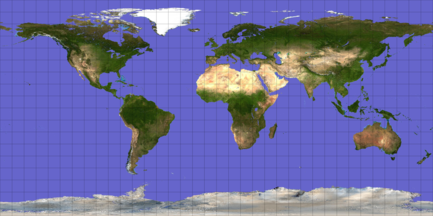
\includegraphics[scale=0.24]{../common/platecarre_thumb.png}  }
\subfigure[Mercator]{
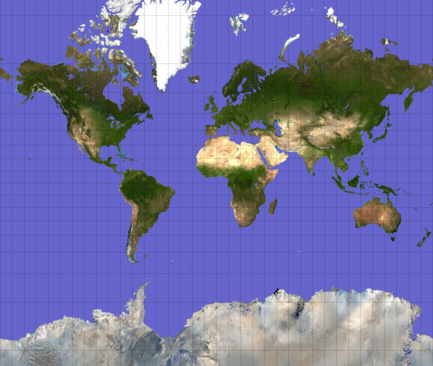
\includegraphics[scale=0.24]{../common/mercator_thumb.png}  }

\subfigure[Gall-Peters]{
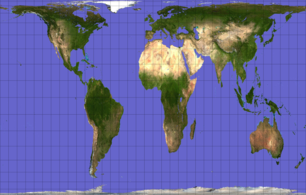
\includegraphics[scale=0.24]{../common/gallpeters_thumb.png} }
\subfigure[Azimuthal Equidistant]{
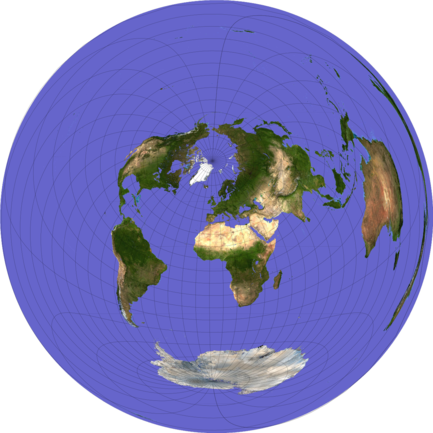
\includegraphics[scale=0.24]{../common/aziequi_thumb.png} }

\subfigure[Gnomonic]{
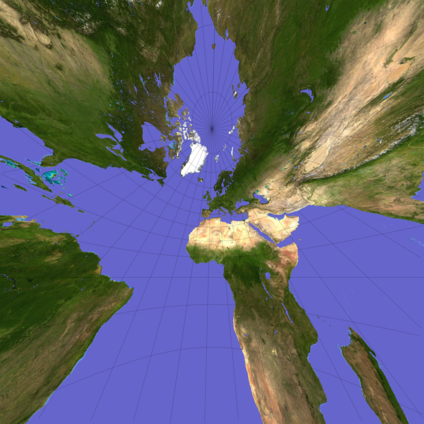
\includegraphics[scale=0.24]{../common/gnomo_thumb.png} }
\subfigure[Mollweide]{
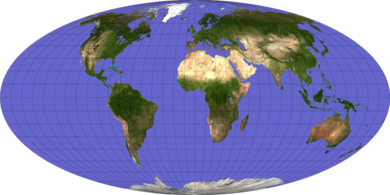
\includegraphics[scale=0.24]{../common/mollweide_thumb.png} }

\caption{Die entsprechend skalierten Poster der Kartenabbildungen.}
\end{center}
\end{figure}

\begin{figure}[ht]
\begin{center}
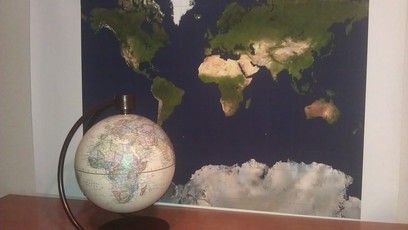
\includegraphics[width=0.6\textwidth]{../common/globe.jpg}
\caption{Der Globus.}
\label{fig-globus}
\end{center}
\end{figure}

\begin{figure}[ht]
\begin{center}
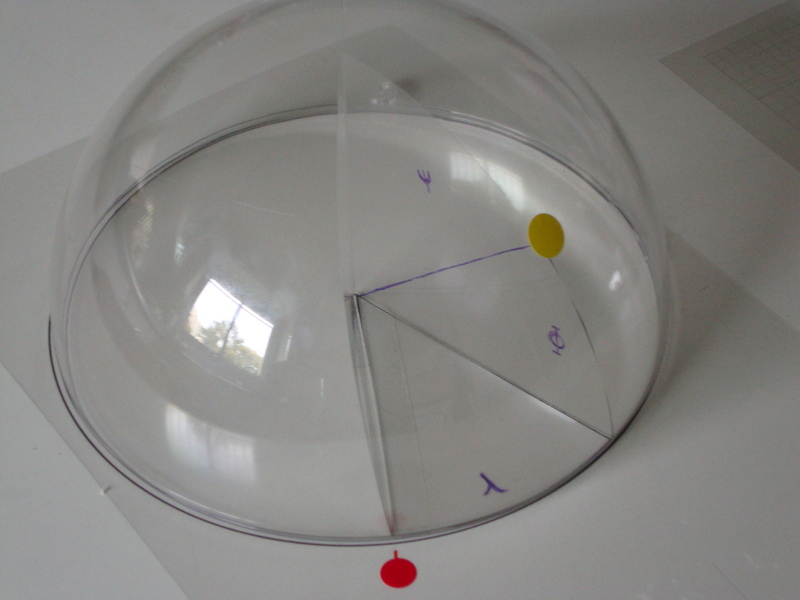
\includegraphics[width=0.6\textwidth]{../common/latlon.jpg}
\caption{Halbkugel zur Veranschaulichung von Längen-- und Breitengrad.}
\label{fig-halbkugel}
\end{center}
\end{figure}


\begin{figure}[ht]
\begin{center}

\subfigure{ 
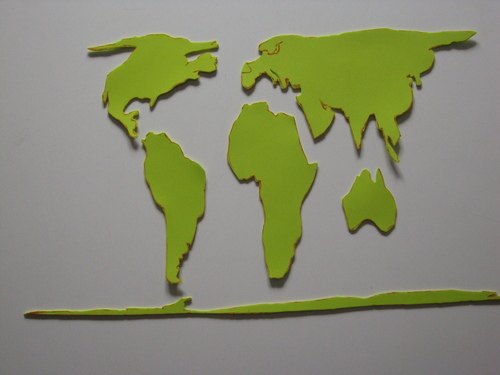
\includegraphics[scale=0.3]{../common/peters_foamy.jpg}  }
\subfigure{
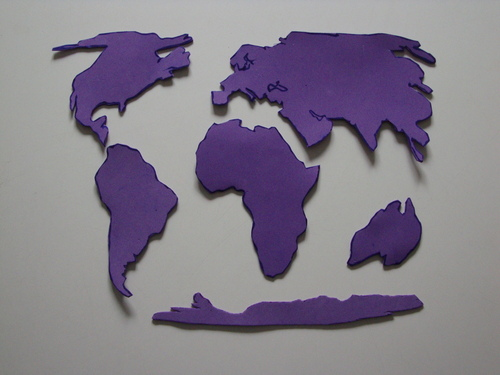
\includegraphics[scale=0.3]{../common/mollweide_foamy.jpg}  }
\subfigure{
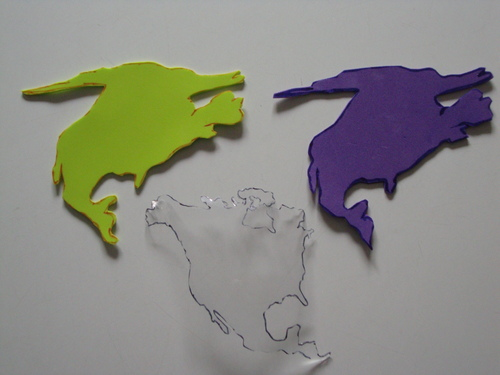
\includegraphics[scale=0.3]{../common/profiles.jpg} }

\caption{Schablonen der Kontinente.}
\label{fig-kontinente}
\end{center}
\end{figure}


\begin{figure}[ht]
\begin{center}
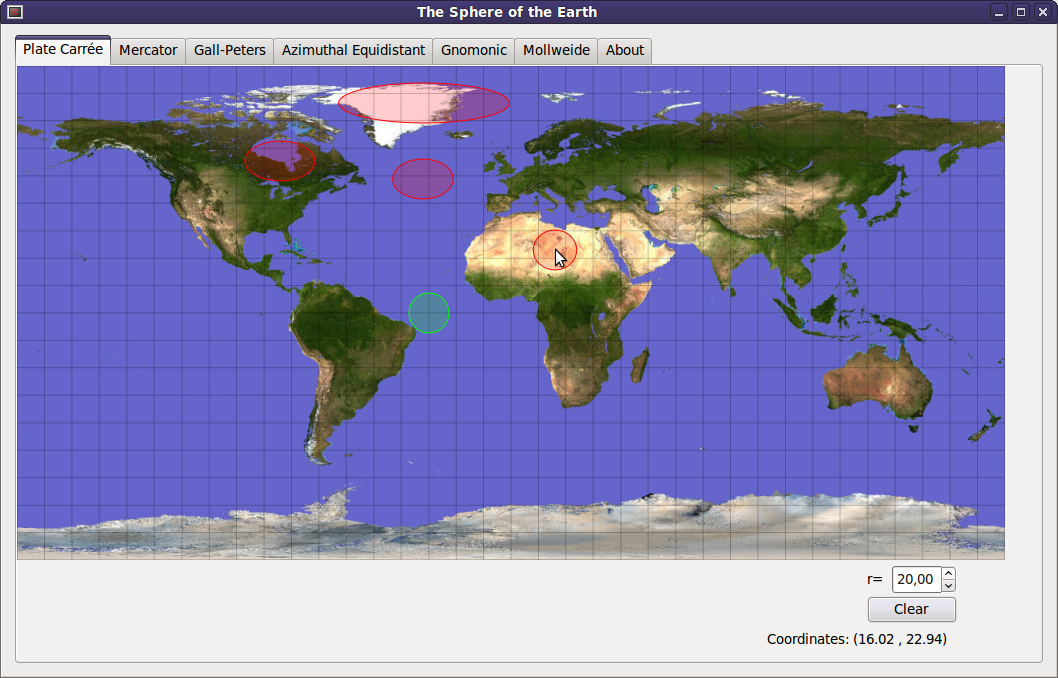
\includegraphics[width=0.8\textwidth]{../common/soe1.png}
\caption{Ein Screenshot des Programms.}
\end{center}
\end{figure}
 
 \begin{figure}[ht]
\begin{center}
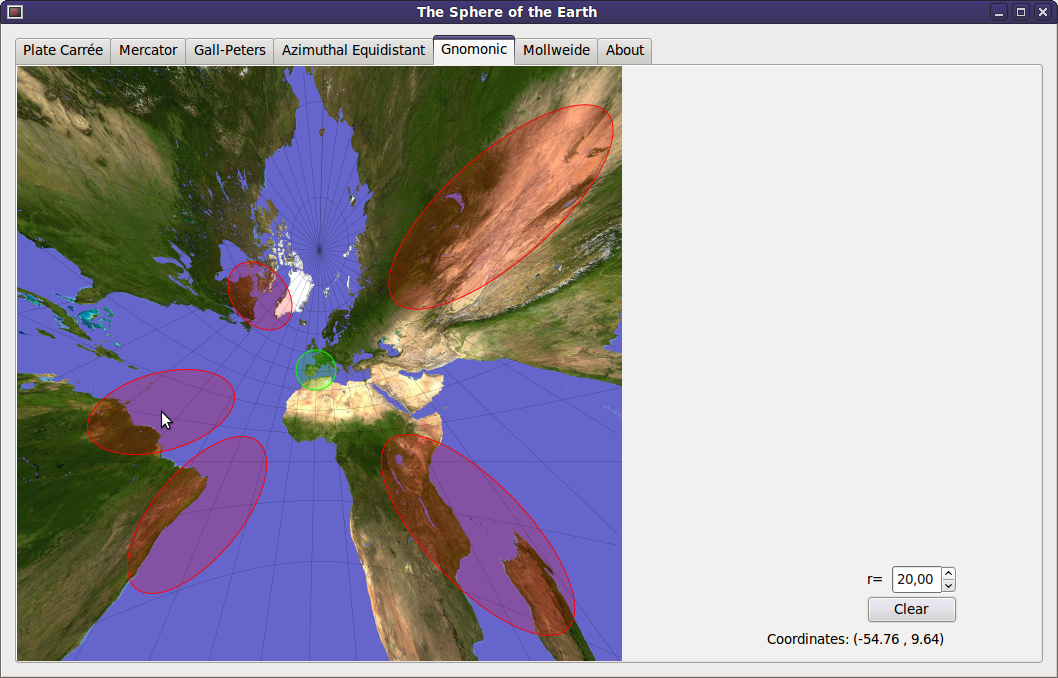
\includegraphics[width=0.8\textwidth]{../common/soe2.png}
\caption{Ein Screenshot des Programms.}
\end{center}
\end{figure}

 
 \begin{figure}[ht]
\begin{center}
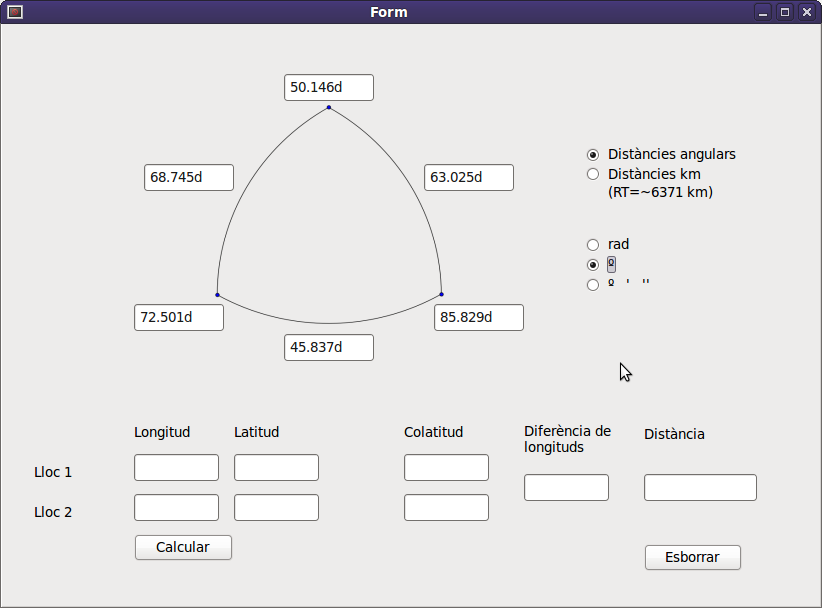
\includegraphics[width=0.8\textwidth]{../common/triang.png}
\caption{Ein Screenshot des Programms zur Berechnung der Kugeldreiecke (in Entwicklung).} 
\label{fig-sphtri}
\end{center}
\end{figure}
 
 \begin{figure}[ht]
\begin{center}
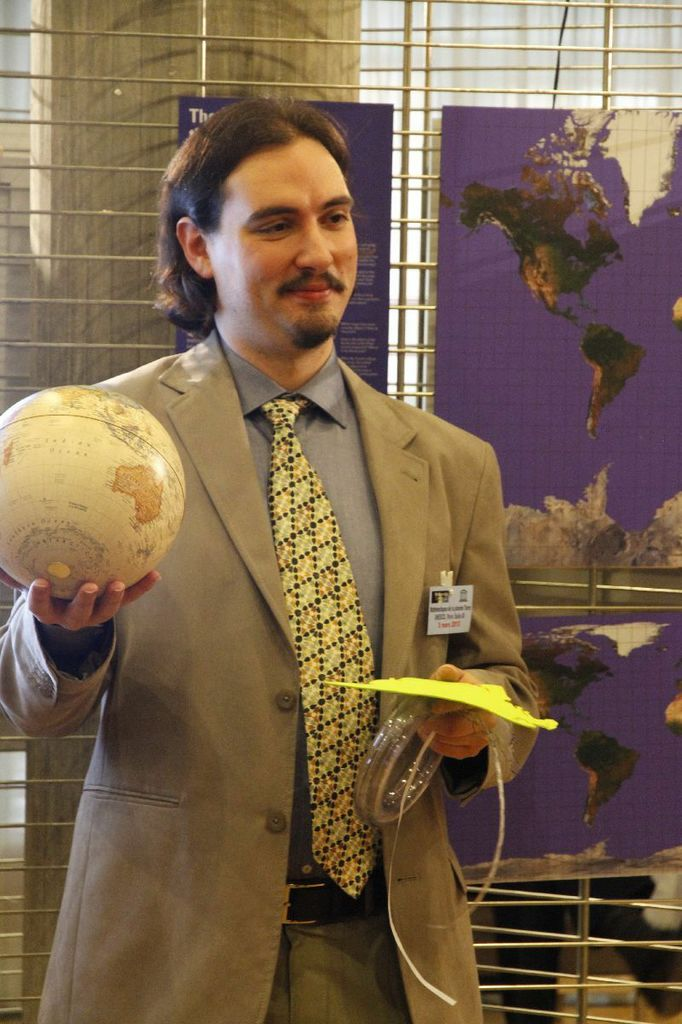
\includegraphics[width=0.8\textwidth]{../common/karten_der_erde.jpg}
\caption{Daniel Ramos bei der Präsentation des Exponats.} 
\end{center}
\end{figure}
 
\end{document}

